% Options for packages loaded elsewhere
\PassOptionsToPackage{unicode}{hyperref}
\PassOptionsToPackage{hyphens}{url}
\PassOptionsToPackage{dvipsnames,svgnames,x11names}{xcolor}
%
\documentclass[
  letterpaper,
  DIV=11,
  numbers=noendperiod]{scrreport}

\usepackage{amsmath,amssymb}
\usepackage{lmodern}
\usepackage{iftex}
\ifPDFTeX
  \usepackage[T1]{fontenc}
  \usepackage[utf8]{inputenc}
  \usepackage{textcomp} % provide euro and other symbols
\else % if luatex or xetex
  \usepackage{unicode-math}
  \defaultfontfeatures{Scale=MatchLowercase}
  \defaultfontfeatures[\rmfamily]{Ligatures=TeX,Scale=1}
\fi
% Use upquote if available, for straight quotes in verbatim environments
\IfFileExists{upquote.sty}{\usepackage{upquote}}{}
\IfFileExists{microtype.sty}{% use microtype if available
  \usepackage[]{microtype}
  \UseMicrotypeSet[protrusion]{basicmath} % disable protrusion for tt fonts
}{}
\makeatletter
\@ifundefined{KOMAClassName}{% if non-KOMA class
  \IfFileExists{parskip.sty}{%
    \usepackage{parskip}
  }{% else
    \setlength{\parindent}{0pt}
    \setlength{\parskip}{6pt plus 2pt minus 1pt}}
}{% if KOMA class
  \KOMAoptions{parskip=half}}
\makeatother
\usepackage{xcolor}
\setlength{\emergencystretch}{3em} % prevent overfull lines
\setcounter{secnumdepth}{5}
% Make \paragraph and \subparagraph free-standing
\ifx\paragraph\undefined\else
  \let\oldparagraph\paragraph
  \renewcommand{\paragraph}[1]{\oldparagraph{#1}\mbox{}}
\fi
\ifx\subparagraph\undefined\else
  \let\oldsubparagraph\subparagraph
  \renewcommand{\subparagraph}[1]{\oldsubparagraph{#1}\mbox{}}
\fi

\usepackage{color}
\usepackage{fancyvrb}
\newcommand{\VerbBar}{|}
\newcommand{\VERB}{\Verb[commandchars=\\\{\}]}
\DefineVerbatimEnvironment{Highlighting}{Verbatim}{commandchars=\\\{\}}
% Add ',fontsize=\small' for more characters per line
\usepackage{framed}
\definecolor{shadecolor}{RGB}{241,243,245}
\newenvironment{Shaded}{\begin{snugshade}}{\end{snugshade}}
\newcommand{\AlertTok}[1]{\textcolor[rgb]{0.68,0.00,0.00}{#1}}
\newcommand{\AnnotationTok}[1]{\textcolor[rgb]{0.37,0.37,0.37}{#1}}
\newcommand{\AttributeTok}[1]{\textcolor[rgb]{0.40,0.45,0.13}{#1}}
\newcommand{\BaseNTok}[1]{\textcolor[rgb]{0.68,0.00,0.00}{#1}}
\newcommand{\BuiltInTok}[1]{\textcolor[rgb]{0.00,0.23,0.31}{#1}}
\newcommand{\CharTok}[1]{\textcolor[rgb]{0.13,0.47,0.30}{#1}}
\newcommand{\CommentTok}[1]{\textcolor[rgb]{0.37,0.37,0.37}{#1}}
\newcommand{\CommentVarTok}[1]{\textcolor[rgb]{0.37,0.37,0.37}{\textit{#1}}}
\newcommand{\ConstantTok}[1]{\textcolor[rgb]{0.56,0.35,0.01}{#1}}
\newcommand{\ControlFlowTok}[1]{\textcolor[rgb]{0.00,0.23,0.31}{#1}}
\newcommand{\DataTypeTok}[1]{\textcolor[rgb]{0.68,0.00,0.00}{#1}}
\newcommand{\DecValTok}[1]{\textcolor[rgb]{0.68,0.00,0.00}{#1}}
\newcommand{\DocumentationTok}[1]{\textcolor[rgb]{0.37,0.37,0.37}{\textit{#1}}}
\newcommand{\ErrorTok}[1]{\textcolor[rgb]{0.68,0.00,0.00}{#1}}
\newcommand{\ExtensionTok}[1]{\textcolor[rgb]{0.00,0.23,0.31}{#1}}
\newcommand{\FloatTok}[1]{\textcolor[rgb]{0.68,0.00,0.00}{#1}}
\newcommand{\FunctionTok}[1]{\textcolor[rgb]{0.28,0.35,0.67}{#1}}
\newcommand{\ImportTok}[1]{\textcolor[rgb]{0.00,0.46,0.62}{#1}}
\newcommand{\InformationTok}[1]{\textcolor[rgb]{0.37,0.37,0.37}{#1}}
\newcommand{\KeywordTok}[1]{\textcolor[rgb]{0.00,0.23,0.31}{#1}}
\newcommand{\NormalTok}[1]{\textcolor[rgb]{0.00,0.23,0.31}{#1}}
\newcommand{\OperatorTok}[1]{\textcolor[rgb]{0.37,0.37,0.37}{#1}}
\newcommand{\OtherTok}[1]{\textcolor[rgb]{0.00,0.23,0.31}{#1}}
\newcommand{\PreprocessorTok}[1]{\textcolor[rgb]{0.68,0.00,0.00}{#1}}
\newcommand{\RegionMarkerTok}[1]{\textcolor[rgb]{0.00,0.23,0.31}{#1}}
\newcommand{\SpecialCharTok}[1]{\textcolor[rgb]{0.37,0.37,0.37}{#1}}
\newcommand{\SpecialStringTok}[1]{\textcolor[rgb]{0.13,0.47,0.30}{#1}}
\newcommand{\StringTok}[1]{\textcolor[rgb]{0.13,0.47,0.30}{#1}}
\newcommand{\VariableTok}[1]{\textcolor[rgb]{0.07,0.07,0.07}{#1}}
\newcommand{\VerbatimStringTok}[1]{\textcolor[rgb]{0.13,0.47,0.30}{#1}}
\newcommand{\WarningTok}[1]{\textcolor[rgb]{0.37,0.37,0.37}{\textit{#1}}}

\providecommand{\tightlist}{%
  \setlength{\itemsep}{0pt}\setlength{\parskip}{0pt}}\usepackage{longtable,booktabs,array}
\usepackage{calc} % for calculating minipage widths
% Correct order of tables after \paragraph or \subparagraph
\usepackage{etoolbox}
\makeatletter
\patchcmd\longtable{\par}{\if@noskipsec\mbox{}\fi\par}{}{}
\makeatother
% Allow footnotes in longtable head/foot
\IfFileExists{footnotehyper.sty}{\usepackage{footnotehyper}}{\usepackage{footnote}}
\makesavenoteenv{longtable}
\usepackage{graphicx}
\makeatletter
\def\maxwidth{\ifdim\Gin@nat@width>\linewidth\linewidth\else\Gin@nat@width\fi}
\def\maxheight{\ifdim\Gin@nat@height>\textheight\textheight\else\Gin@nat@height\fi}
\makeatother
% Scale images if necessary, so that they will not overflow the page
% margins by default, and it is still possible to overwrite the defaults
% using explicit options in \includegraphics[width, height, ...]{}
\setkeys{Gin}{width=\maxwidth,height=\maxheight,keepaspectratio}
% Set default figure placement to htbp
\makeatletter
\def\fps@figure{htbp}
\makeatother

\KOMAoption{captions}{tableheading}
\makeatletter
\@ifpackageloaded{tcolorbox}{}{\usepackage[many]{tcolorbox}}
\@ifpackageloaded{fontawesome5}{}{\usepackage{fontawesome5}}
\definecolor{quarto-callout-color}{HTML}{909090}
\definecolor{quarto-callout-note-color}{HTML}{0758E5}
\definecolor{quarto-callout-important-color}{HTML}{CC1914}
\definecolor{quarto-callout-warning-color}{HTML}{EB9113}
\definecolor{quarto-callout-tip-color}{HTML}{00A047}
\definecolor{quarto-callout-caution-color}{HTML}{FC5300}
\definecolor{quarto-callout-color-frame}{HTML}{acacac}
\definecolor{quarto-callout-note-color-frame}{HTML}{4582ec}
\definecolor{quarto-callout-important-color-frame}{HTML}{d9534f}
\definecolor{quarto-callout-warning-color-frame}{HTML}{f0ad4e}
\definecolor{quarto-callout-tip-color-frame}{HTML}{02b875}
\definecolor{quarto-callout-caution-color-frame}{HTML}{fd7e14}
\makeatother
\makeatletter
\makeatother
\makeatletter
\makeatother
\makeatletter
\@ifpackageloaded{caption}{}{\usepackage{caption}}
\AtBeginDocument{%
\ifdefined\contentsname
  \renewcommand*\contentsname{Table of contents}
\else
  \newcommand\contentsname{Table of contents}
\fi
\ifdefined\listfigurename
  \renewcommand*\listfigurename{List of Figures}
\else
  \newcommand\listfigurename{List of Figures}
\fi
\ifdefined\listtablename
  \renewcommand*\listtablename{List of Tables}
\else
  \newcommand\listtablename{List of Tables}
\fi
\ifdefined\figurename
  \renewcommand*\figurename{Figure}
\else
  \newcommand\figurename{Figure}
\fi
\ifdefined\tablename
  \renewcommand*\tablename{Table}
\else
  \newcommand\tablename{Table}
\fi
}
\@ifpackageloaded{float}{}{\usepackage{float}}
\floatstyle{ruled}
\@ifundefined{c@chapter}{\newfloat{codelisting}{h}{lop}}{\newfloat{codelisting}{h}{lop}[chapter]}
\floatname{codelisting}{Listing}
\newcommand*\listoflistings{\listof{codelisting}{List of Listings}}
\makeatother
\makeatletter
\@ifpackageloaded{caption}{}{\usepackage{caption}}
\@ifpackageloaded{subcaption}{}{\usepackage{subcaption}}
\makeatother
\makeatletter
\@ifpackageloaded{tcolorbox}{}{\usepackage[many]{tcolorbox}}
\makeatother
\makeatletter
\@ifundefined{shadecolor}{\definecolor{shadecolor}{rgb}{.97, .97, .97}}
\makeatother
\makeatletter
\makeatother
\ifLuaTeX
  \usepackage{selnolig}  % disable illegal ligatures
\fi
\IfFileExists{bookmark.sty}{\usepackage{bookmark}}{\usepackage{hyperref}}
\IfFileExists{xurl.sty}{\usepackage{xurl}}{} % add URL line breaks if available
\urlstyle{same} % disable monospaced font for URLs
\hypersetup{
  pdftitle={Programming for Data Science},
  pdfauthor={Rafael C. Alvarado},
  colorlinks=true,
  linkcolor={blue},
  filecolor={Maroon},
  citecolor={Blue},
  urlcolor={Blue},
  pdfcreator={LaTeX via pandoc}}

\title{Programming for Data Science}
\author{Rafael C. Alvarado}
\date{5/8/21}

\begin{document}
\maketitle
\ifdefined\Shaded\renewenvironment{Shaded}{\begin{tcolorbox}[borderline west={3pt}{0pt}{shadecolor}, sharp corners, frame hidden, enhanced, boxrule=0pt, interior hidden, breakable]}{\end{tcolorbox}}\fi

\renewcommand*\contentsname{Table of contents}
{
\hypersetup{linkcolor=}
\setcounter{tocdepth}{2}
\tableofcontents
}
\part{Preface}

Welcome to Programming for Data Science, a collection of materials
designed to support the course DS 5100 in the Data Science curriculum at
UVA.

In this course, you will develop skills in Python and R Programming, as
well as how to use the command line and GitHub.

The objective of this course is to introduce essential programming
concepts, structures, and techniques.

You will gain confidence in not only reading code, but learning what it
means to write good quality code.

Additionally, essential and complementary topics are taught, such as
testing and debugging, exception handling, and an introduction to
visualization.

\part{Getting Started}

During the technical orientation, you set up a GitHub account.

You also spent a little time browsing a sample repository, which you may
wish to revisit:

https://github.com/UVADS/orientation-technical

You also should be able check off the following items:

\begin{itemize}
\tightlist
\item
  Understand the difference between Git and GitHub.
\item
  Understand the purpose of Git and Github for data science work.
\item
  Ensure Git is installed on your computer.
\item
  Understand how to find a repository on GitHub.
\end{itemize}

\hypertarget{about-rivanna}{%
\chapter{About Rivanna}\label{about-rivanna}}

\hypertarget{introduction}{%
\section{Introduction}\label{introduction}}

A useful infrastructural resource for this course is Rivanna, UVA's
high-performance computing (HPC) cluster. Each student has an account on
Rivanna and access to resources there based on participation in this
course. We will use Rivanna in our class for both Python and R.~

This page describes some of the tools available for your use in this
course. For information about Rivanna, see~this introduction. Resources
for getting help, including a knowledge base and ticket system, are
found at~\href{http://www.rc.virginia.edu/support/}{the Support Option's
Page} on UVA's Research Computing website.

You may need to use VPN to access Rivanna from an off-grounds location.
To install VPN on your computer, go to the~ITS VPN page~for
instructions. Note that you should connect to ``UVA Anywhere,'' not to
any of the higher security options. Course Allocation

This course has been allocated compute and space resources on Rivanna.
The names of the resources are given below. The allocation ID needs to
be entered to access certain tools. The storage path is accessible to
you on the remote server.

\begin{itemize}
\tightlist
\item
  Allocation ID: \texttt{msds\_ds5100}
\item
  Storage path: \texttt{/project/MSDS\_DS5100}~ (Don't use unless
  directed to.)
\end{itemize}

\hypertarget{tools}{%
\section{Tools~}\label{tools}}

UVA Research Computing provides you with a suite of tools to access
Rivanna. These tools are accessible through the menu on the
UVA~OpenOnDemand Dashboard page. Below are some brief descriptions of
the tools.

\textbf{File Explorer}. A web-based GUI to access the file system of the
remote server. Can be used to create, move, and delete directories and
files, and to edit the contents of files (see Editor). You can also
upload and download files through this interface. The File Explorer is
useful to view your remote content and manage files and directories
without having to use the command line. Note that not all operations can
be performed through this interface.

Find under ``Files'' in the menu.~

\textbf{Editor}. A web-based text editor launched from the File Explorer
to view and edit text files on the remote server.~ Although not as
sophisticated as VS Code (below), this is very useful for editing data
and code files without having to use a command line editor. One
advantage over VS Code is that it does not need to be launched -- which
means it does not time out like the Interactive Apps listed below.

The Editor is launched from the File Explorer.

\textbf{SSH Shell Access (Terminal)}.~Access to the command line of the
remote server.~ Use this to open a terminal window to perform Linux
commands directly.~ Note that It is necessary to use a terminal to
install and run certain programs on the remote server.

Find under ``Clusters'' in the menu.~

You can also access the remote command line via SSH on your local
computer. Just enter the following on the command line of either a PC or
Mac:

\begin{Shaded}
\begin{Highlighting}[]
\FunctionTok{ssh} \AttributeTok{{-}Y} \OperatorTok{\textless{}}\NormalTok{userid}\OperatorTok{\textgreater{}}\NormalTok{@hpc.rivanna.virginia.edu}
\end{Highlighting}
\end{Shaded}

Replace~\texttt{\textless{}userid\textgreater{}}~with your UVA Net ID,
e.g.~\texttt{abc2x}.~

Be suer to be running VPN if you are accessing Rivanna from an
off-grounds location.

\hypertarget{interactive-spps}{%
\section{Interactive Spps}\label{interactive-spps}}

These tools must be launched by specifying a set of parameters,
including the allocation you are using. They are also timed and will
close when time is up. Be sure to give yourself enough time when
launching these, and to be aware of how much time you have when working.

Note also that you should allocate the fewest resources necessary to do
the work you plan to do. This saves resources on the remote host, but
also allows your app to launch more quickly. If you ask for an excessive
amount of resources, you may wait a long time (e.g.~hours) to have your
app launched.

\textbf{Desktop}.~Access to a GUI desktop to the remote server. This
provides a access to various applications on the server, including a web
browser, a file explorer, and terminal windows.~ Using this is not
necessary if you can get by with the tools listed above.

Find under ``Interactive Apps \textgreater{} Desktop'' in the menu.

\textbf{VS Code}. Access to Visual Studio Code on the remote server.
This is a fully functional instance of the IDE.

Find under ``Interactive Apps \textgreater{} Code Server'' in the menu.

\textbf{Jupyter}.~Access to Jupyter Lab on the remote server. Find under
``Interactive Apps \textgreater{} Jupyter Lab'' in the menu.

\textbf{RStudio}. Access to Jupyter Lab on the remote server.

Find under ``Interactive Apps \textgreater{} RStudio Server'' in the
menu.

\hypertarget{for-more-information}{%
\section{For More Information}\label{for-more-information}}

UVA's Research Computing unit provides resources for learning how to use
Rivanna. Here are two slide decks that you may find useful:

\begin{itemize}
\tightlist
\item
  Introduction to Rivanna
\item
  Using Rivanna from the Command Line
\end{itemize}

\hypertarget{using-unix}{%
\chapter{Using Unix}\label{using-unix}}

\hypertarget{introduction-1}{%
\section{Introduction}\label{introduction-1}}

The Unix family of operating systems provide users with~a command line
interface~(CLI) to execute commands and get things done. They also,
typically provide GUIs but we won't go into those here.

The Unix family includes all varieties of Linux and the Mac OS (which is
based on FreeBSD).

The command line that you actually interact with -- the set of commands
available to you -- is called a~shell, and there are several shells that
you can run on your system. The most typical shell in use today is
called~bash~which stands for Bourne Again Shell, since it is an improved
version of~bsh~(The Bourne Shell). New versions of MacOS use the Z shell
(zsh). The commands in these two shells are mostly similar, but there
are subtle differences.

Windows has shells too for its command line interface. The default shell
is DOS, but is also has~PowerShell~ as an advanced (and very capable)
option.

For more information, check out these resources:

\begin{itemize}
\tightlist
\item
  UVA Research
  Computing's~\href{https://learning.rc.virginia.edu/notes/unix-tutorial/}{Unix
  tutorial}.
\item
  Newham,
  2005,~\href{https://learning.oreilly.com/library/view/learning-the-bash/0596009658/}{Learning
  the bash Shell}, O'Reilly Media.
\item
  Jeroen Janssens,
  2021,~\href{https://datascienceatthecommandline.com/2e/}{Data Science
  From the Command Line},~O'Reilly Media.
\item
  Neal Stephenson,
  1999,~\href{http://project.cyberpunk.ru/lib/in_the_beginning_was_the_command_line/}{In
  the Beginning Was The Command Line}.
  (\href{http://public-library.uk/ebooks/23/31.pdf}{PDF version}.)
\end{itemize}

\hypertarget{basic-commands}{%
\section{Basic Commands}\label{basic-commands}}

In this course, you don't need to know very many Unix shell commands,
but you should be~comfortable~working from the command line to perform
basic tasks. This is because~some things can only be performed from the
command line, such as installing some essential software. Here is a list
of basic commands.

Navigating filesystems and managing directories:

\begin{itemize}
\tightlist
\item
  \texttt{cd} -- change directory
\item
  \texttt{pwd} -- show the current directory
\item
  \texttt{ln} -- make links and symlinks to files and directories
\item
  \texttt{mkdir} -- make new directory
\item
  \texttt{rmdir} -- remove directories in Unix
\end{itemize}

Navigating filesystem and managing files and access permissions:

\begin{itemize}
\tightlist
\item
  \texttt{ls} -- list files and directories
\item
  \texttt{cp} -- copy files (work in progress)
\item
  \texttt{rm} -- remove files and directories (work in progress)
\item
  \texttt{mv} -- rename or move files and directories to another
  location
\item
  \texttt{chmod} -- change file/directory access permissions
\item
  \texttt{chown} -- change file/directory ownership
\end{itemize}

\hypertarget{text-file-commands}{%
\section{Text file commands}\label{text-file-commands}}

Most of important configuration in Unix is in plain text files, these
commands will let you quickly inspect files or view logs:

\begin{itemize}
\tightlist
\item
  \texttt{cat} -- concatenate files and show contents to the standard
  output
\item
  \texttt{more} -- basic pagination when viewing text files or parsing
  Unix commands output
\item
  \texttt{less} -- an improved pagination tool for viewing text files
  (better than more command)
\item
  \texttt{head} -- show the first 10 lines of text file (you can specify
  any number of lines)
\item
  \texttt{tail} -- show the last 10 lines of text file (any number can
  be specified)
\item
  \texttt{grep} -- search for patterns in text files
\end{itemize}

\hypertarget{miscellaneous}{%
\section{Miscellaneous}\label{miscellaneous}}

\begin{itemize}
\tightlist
\item
  \texttt{clear} -- clear screen
\item
  \texttt{history} -- show history of previous commands
\end{itemize}

\hypertarget{command-line-cool}{%
\section{Command Line Cool}\label{command-line-cool}}

Although we will not be using the command line to this degree, you
should know that it is a powerful environment for doing data science
work. The book~\href{https://datascienceatthecommandline.com/2e/}{Data
Science from the Command Line}~makes the case for using the command line
to perform many tasks that we often perform with more resource intensive
(i.e.~bloated) tools such as Python and R.~ At some point in your early
DS career, you may want to look at this. The book itself is also a great
introduction to data science!

\includegraphics{https://datascienceatthecommandline.com/2e/images/cover-small.png}

One last thing -- for fun you may want to read Neal
Stephenson's~\href{http://project.cyberpunk.ru/lib/in_the_beginning_was_the_command_line/}{``In
the Beginning Was The Command Line''}, a kind of cyberpunk history of
the topic. Stephenson, by the way, is the author who coined the term
``metaverse'' in the novel~\emph{Snowcrash}.

\hypertarget{data-and-code}{%
\chapter{Data and Code}\label{data-and-code}}

An important principle for writing effective and intelligible code is
that code should be simple --- to quote Einstein, as simple as possible
but no simpler.

\begin{itemize}
\tightlist
\item
  A contributing factor to code simplicity is how it is related to the
  data it is designed to process.
\item
  This relationship depends largely on how the data are structured.
\item
  A program is always written with data in mind --- what kind of data it
  is and how it is structured.
\end{itemize}

\hypertarget{simplicity-of-code-follows-from-the-structure-of-data}{%
\section{Simplicity of code follows from the structure of
data}\label{simplicity-of-code-follows-from-the-structure-of-data}}

There is a view among programmers which, although not orthodoxy, is
commonplace.

\begin{itemize}
\tightlist
\item
  It is the idea that the complexity of a program --- its algorithms ---
  is a function of the quality of the data structure it processes.
\item
  If a data structure is not well designed, algorithms may be
  excessively complex and hard to understand.
\item
  However if a data structure is well designed, the algorithms that
  process them are more robust and intelligible.
\end{itemize}

\hypertarget{supporting-references}{%
\section{Supporting References}\label{supporting-references}}

Consider these quotes cited in an essay on
\href{https://medium.com/webdevops/data-structures-548cbea9c520}{Data
Structures}. by Igor Budasov, reproduced here:

Here's \href{https://lwn.net/Articles/193245/}{a quote from Linus
Torvalds in 2006}:

\begin{quote}
I'm a huge proponent of designing your code around the data, rather than
the other way around, and I think it's one of the reasons git has been
fairly successful . . . I will, in fact, claim that the difference
between a bad programmer and a good one is whether he considers his
{[}sic{]} code or his data structures more important. Bad programmers
worry about the code. Good programmers worry about data structures and
their relationships.
\end{quote}

Which sounds a lot like
\href{http://www.catb.org/~esr/writings/taoup/html/ch01s06.html}{Eric
Raymond's ``Rule of Representation'' from 2003}:

\begin{quote}
Fold knowledge into data, so program logic can be stupid and robust.
\end{quote}

Which was just his summary of ideas like
\href{http://doc.cat-v.org/bell_labs/pikestyle}{this one from Rob Pike
in 1989}:

\begin{quote}
Data dominates. If you've chosen the right data structures and organized
things well, the algorithms will almost always be self-evident. Data
structures, not algorithms, are central to programming.
\end{quote}

Which cites
\href{https://archive.org/stream/mythicalmanmonth00fred/mythicalmanmonth00fred_djvu.txt}{Fred
Brooks from 1975}:

\begin{quote}
\textbf{Representation is the Essence of Programming}\\
\strut \\
Beyond craftsmanship lies invention, and it is here that lean, spare,
fast programs are born. Almost always these are the result of strategic
breakthrough rather than tactical cleverness. Sometimes the strategic
breakthrough will be a new algorithm, such as the Cooley-Tukey Fast
Fourier Transform or the substitution of an n log n sort for an n 2 set
of comparisons.
\end{quote}

\begin{quote}
\textbf{Much more often, strategic breakthrough will come from redoing
the representation of the data or tables.} This is where the heart of
your program lies. Show me your flowcharts and conceal your tables, and
I shall be continued to be mystified. Show me your tables, and I won't
usually need your flowcharts; they'll be obvious.
\end{quote}

\hypertarget{python-object-types}{%
\chapter{Python Object Types}\label{python-object-types}}

Python is organized into a hierarchy of object types. Sometimes, these
are just call \textbf{types}.

Objects are the basic unit out of which the language is constructed.

We'll learn about objects later -- what they are and how to create your
own -- but for now just understand that they have two main things
associated with them:

\begin{itemize}
\tightlist
\item
  First, they can contain \textbf{data}.
\item
  Second, they can have \textbf{behaviors}, frequently in relation to
  the data they contain.
\end{itemize}

Data types and data structures are kinds of objects.

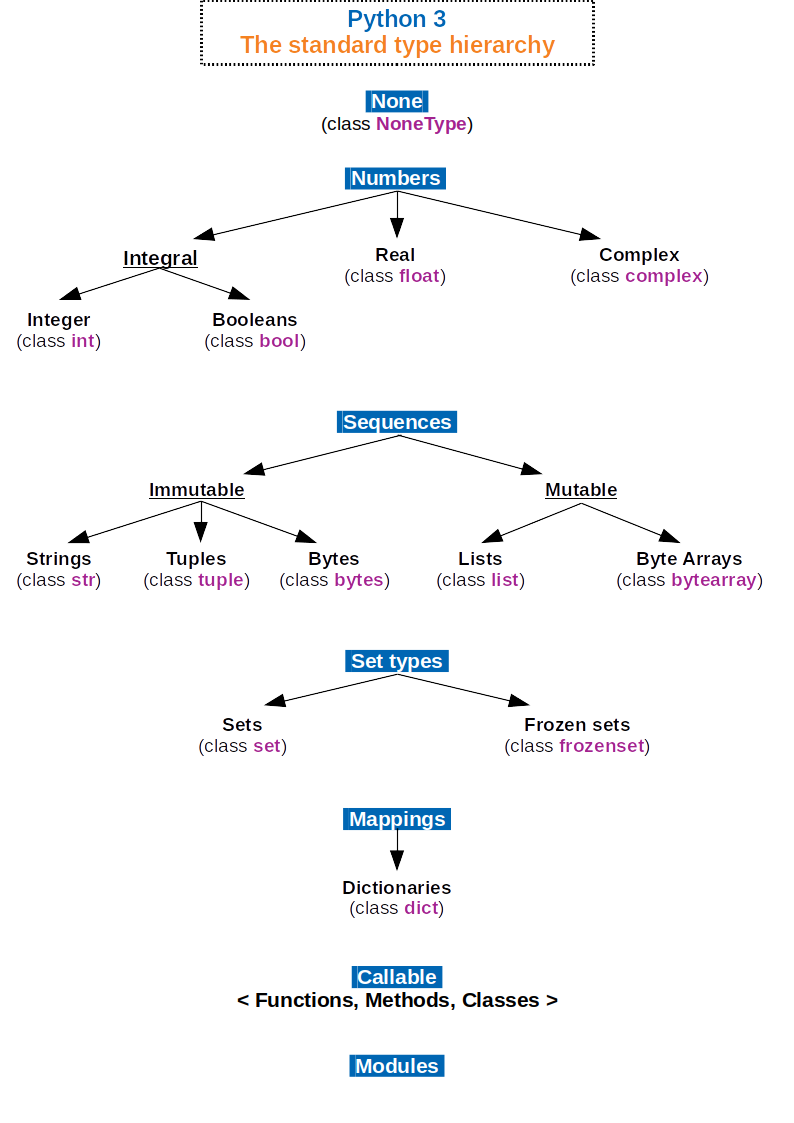
\includegraphics{topics/media/Python_3._The_standard_type_hierarchy.png}

\hypertarget{activity-using-git-and-github}{%
\chapter{Activity: Using Git and
GitHub}\label{activity-using-git-and-github}}

Git and GitHub are two tools that work together, but it is important to
understand what each does and how they are different to each other.

Here are some basic things to know:

\begin{enumerate}
\def\labelenumi{\arabic{enumi}.}
\tightlist
\item
  Git is a stand-alone version control system that runs on a variety of
  platforms, including Linux, MacOS, and Windows.
\item
  GitHub is a company that offers a cloud-based Git repository hosting
  service that makes it easy to use Git for version control,
  collaboration, and sharing code. This service is offered through a
  website.
\item
  There are other Git hosting services out there, including GitLab, and
  open source tool that can be installed on a local server.
\item
  GitHub builds on top of Git and adds some functionality to it, while
  Git can interact with GitHub through actions like cloning, pushing,
  and pulling. However, Git does not require GitHub to function.
\item
  Git does not have a fork command. GitHub (and other hosting services
  such as GitLab) have added this command as a convenient way to copy
  repositories.
\end{enumerate}

\hypertarget{using-git-and-github-together}{%
\section{Using Git and GitHub
Together}\label{using-git-and-github-together}}

\begin{figure}

{\centering 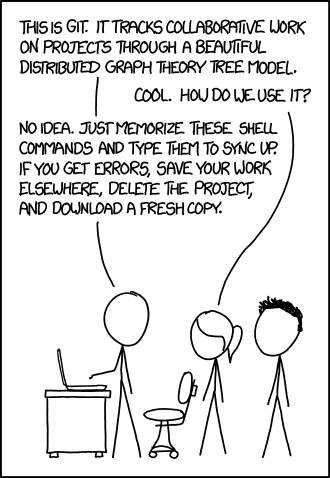
\includegraphics{modules/../media/xkcd-git.png}

}

\caption{XKCD \#1597}

\end{figure}

\href{https://xkcd.com/1597}{Source}

A basic series of actions one continually makes with Git are the
following:

\begin{longtable}[]{@{}
  >{\raggedright\arraybackslash}p{(\columnwidth - 4\tabcolsep) * \real{0.2667}}
  >{\raggedright\arraybackslash}p{(\columnwidth - 4\tabcolsep) * \real{0.4333}}
  >{\raggedright\arraybackslash}p{(\columnwidth - 4\tabcolsep) * \real{0.3000}}@{}}
\toprule()
\begin{minipage}[b]{\linewidth}\raggedright
Action
\end{minipage} & \begin{minipage}[b]{\linewidth}\raggedright
Description
\end{minipage} & \begin{minipage}[b]{\linewidth}\raggedright
Command
\end{minipage} \\
\midrule()
\endhead
\textbf{Fork} & Forking a repo makes a copy of someone else's repo in
your GitHub account, which you can now modify. Note: Forking does not
have to be performed if you are not interested in altering the code. You
can clone it directlty. & This is done through GitHub's web interface by
clicking on the Fork button. \\
\textbf{Clone} & Cloning the repo to a workspace to which you have
access, whether a local machine or a remote resource (e.g.~Rivanna). &
\texttt{git\ clone\ \textless{}repo\textgreater{}} \\
\textbf{Add} & Creating or editing a file locally and then adding it to
the list of files git will keep track of. &
\texttt{git\ add\ \textless{}filename\textgreater{}}Note that you may
use wildcards here, e.g.~*, to add more than one file at a time. \\
\textbf{Commit} & Committing the changes made to the file by adding them
to the repo's database of changes. This is accompanied by a brief,
descriptive message of the changes made. &
\texttt{git\ commit\ -m\ "What\ you\ did"} \\
\textbf{Push} & Pushing the changes to the remote repo that you cloned
from. This uploads both the files and the database changes to the repo.
& \texttt{git\ push} \\
\textbf{Pull} & Pulling, i.e.~downloading, any changes that have been
made to the remote repo to your local repo. This usually happens if you
are working in teams on the same project. & \texttt{git\ pull} \\
\textbf{Pull Request} & This is a request made to the owner of the
original repo to pull in the changes you've made to your forked copy. &
This is done through GitHub's web interface. Read the
\href{https://docs.github.com/en/pull-requests}{docs}.~
\includegraphics{modules/../media/pull-request-button.jpg} \\
\textbf{Fetch Upstream} & This refreshes the content of your forked repo
with the content from the original repo. & This is done through GitHub's
web interface. Read the
\href{https://docs.github.com/en/pull-requests/collaborating-with-pull-requests/working-with-forks/syncing-a-fork}{docs}.~
\includegraphics{modules/../media/sync-fork.jpg} \\
\bottomrule()
\end{longtable}

\begin{tcolorbox}[enhanced jigsaw, bottomrule=.15mm, leftrule=.75mm, opacityback=0, toprule=.15mm, colback=white, rightrule=.15mm, left=2mm, coltitle=black, arc=.35mm, breakable, colframe=quarto-callout-note-color-frame, toptitle=1mm, bottomtitle=1mm, title=\textcolor{quarto-callout-note-color}{\faInfo}\hspace{0.5em}{Note}, opacitybacktitle=0.6, titlerule=0mm, colbacktitle=quarto-callout-note-color!10!white]

This is not the only pattern to use with Git. Here is another ---
\href{https://www.tomasbeuzen.com/post/git-fork-branch-pull/}{the Git
Fork-Branch-Pull Workflow}

\end{tcolorbox}

Here is a visualization of the process:

\begin{figure}

{\centering 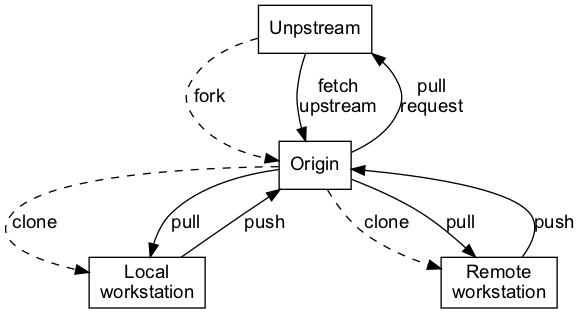
\includegraphics{modules/../media/git.png}

}

\caption{Diagram of common git workflow}

\end{figure}

In this diagram, the dashed lines refer to actions performed only once
for a give repo. Forking and cloning are done to acquire a repo, while
fetch upstream (aka sync fork) and pull requests on the GitHub server,
and pull/push on your local machine, are done repeatedly as you develop
and share code.

Note also that the here ``Remote workstation'' may be confusing; it
means remote relative to your laptop, e.g.~Rivanna, which we sometimes
call local relative to the GitHub repo. In any case, note that these two
copies of the same repo do not communicate with each other directly, but
rather through their common relationship with the GitHub hosted instance
of the repo.

\hypertarget{in-class-activity}{%
\section{In-Class Activity}\label{in-class-activity}}

Let's try this now with our course repo.

Be sure you are inside the course directory we created earlier.

Also, we assume you have already created a GitHub account.

\textbf{\emph{Fork} the course GitHub hosted repository (``repo'') to
your GitHub account.}

Go to https://github.com/ontoligent/DS5100-2023-07-R in your web
browser.

\begin{tcolorbox}[enhanced jigsaw, bottomrule=.15mm, leftrule=.75mm, opacityback=0, toprule=.15mm, colback=white, rightrule=.15mm, left=2mm, coltitle=black, arc=.35mm, breakable, colframe=quarto-callout-note-color-frame, toptitle=1mm, bottomtitle=1mm, title=\textcolor{quarto-callout-note-color}{\faInfo}\hspace{0.5em}{Note}, opacitybacktitle=0.6, titlerule=0mm, colbacktitle=quarto-callout-note-color!10!white]

This is the course repo --- all of the course notebooks and other code
will be available here.~Each week, you will access your course materials
here.

\end{tcolorbox}

Click on the Fork icon in the upper right and follow the prompts to
finish the process.

You should end up at the web page of your newly forked repo.

You will now have a copy of the repo in your GitHub account.

\textbf{\emph{Clone} the forked repo for this course inside of your
course directory on Rivanna.}

Find the green Code button and click on it. You should see something
like this:

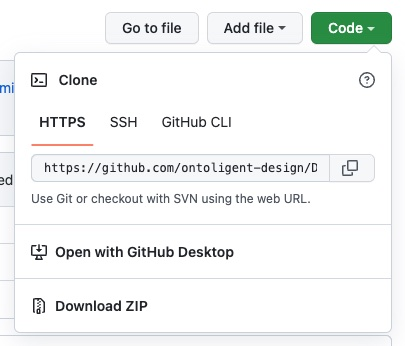
\includegraphics{modules/../media/git-clone.jpg}

Make sure you have selected the SSH option.

\begin{tcolorbox}[enhanced jigsaw, bottomrule=.15mm, leftrule=.75mm, opacityback=0, toprule=.15mm, colback=white, rightrule=.15mm, left=2mm, coltitle=black, arc=.35mm, breakable, colframe=quarto-callout-important-color-frame, toptitle=1mm, bottomtitle=1mm, title=\textcolor{quarto-callout-important-color}{\faExclamation}\hspace{0.5em}{Important}, opacitybacktitle=0.6, titlerule=0mm, colbacktitle=quarto-callout-important-color!10!white]

Note: This requires that you have SSH set up.

\end{tcolorbox}

Then click on the copy icon and paste the value into the following
command:

\begin{Shaded}
\begin{Highlighting}[]
\FunctionTok{git}\NormalTok{ clone https://github.com:}\OperatorTok{\textless{}}\NormalTok{github\_user\_name}\OperatorTok{\textgreater{}}\NormalTok{/DS5100{-}2023{-}07{-}R.git}
\end{Highlighting}
\end{Shaded}

\begin{tcolorbox}[enhanced jigsaw, bottomrule=.15mm, leftrule=.75mm, opacityback=0, toprule=.15mm, colback=white, rightrule=.15mm, left=2mm, coltitle=black, arc=.35mm, breakable, colframe=quarto-callout-important-color-frame, toptitle=1mm, bottomtitle=1mm, title=\textcolor{quarto-callout-important-color}{\faExclamation}\hspace{0.5em}{Important}, opacitybacktitle=0.6, titlerule=0mm, colbacktitle=quarto-callout-important-color!10!white]

Be sure to clone the repo from \emph{your} GitHub account, replacing
\texttt{\textless{}github\_user\_name\textgreater{}} with your GitHub
user name. Do not just cut-and-paste the line above!

\end{tcolorbox}

You now have a copy the course repo to your account on Rivanna.

This will be the directory you created in your pre-class activities
under Documents/.

\textbf{\emph{Create} a new file in your newly cloned repo.}

Go to your command line window on Rivanna.

Use \texttt{cd} to move into the directory just created by the clone
operation.

Move into the directory \texttt{lessons/M01\_GettingStarted/hello}

\begin{tcolorbox}[enhanced jigsaw, bottomrule=.15mm, leftrule=.75mm, opacityback=0, toprule=.15mm, colback=white, rightrule=.15mm, left=2mm, coltitle=black, arc=.35mm, breakable, colframe=quarto-callout-important-color-frame, toptitle=1mm, bottomtitle=1mm, title=\textcolor{quarto-callout-important-color}{\faExclamation}\hspace{0.5em}{Important}, opacitybacktitle=0.6, titlerule=0mm, colbacktitle=quarto-callout-important-color!10!white]

Make sure you are in this directory before proceeding.

\end{tcolorbox}

If you get lost -- for example if you moved around the file system
before this step -- you can cd to the absolute path:

\begin{Shaded}
\begin{Highlighting}[]
\BuiltInTok{cd}\NormalTok{ \textasciitilde{}/Documents/MSDS/DS5100/DS5100{-}2023{-}07{-}R/lessons/M01\_GettingStarted/hello }
\end{Highlighting}
\end{Shaded}

Note that the tilde sign \texttt{\textasciitilde{}} stands for the path
to your home directory.

Using the file editor on Rivanna, create and save new file called
\texttt{\textless{}userid\textgreater{}\_hello.txt}, replacing
\texttt{\textless{}userid\textgreater{}} with your actual user ID,
e.g.~\texttt{rca2t\_hello.txt}.

In the file, introduce yourself by answering the question: What is the
most recent film you watched and enjoyed?

Save the file.

\textbf{\emph{Add} and \emph{commit} the changes you made.}

Now do the following:

\begin{Shaded}
\begin{Highlighting}[]
\FunctionTok{git}\NormalTok{ add }\OperatorTok{\textless{}}\NormalTok{userid}\OperatorTok{\textgreater{}}\NormalTok{\_hello.txt}
\FunctionTok{git}\NormalTok{ commit }\AttributeTok{{-}m} \StringTok{"Created file for class"}
\end{Highlighting}
\end{Shaded}

\textbf{\emph{Push} your new file to the repo on GitHub.}

Since you have SSH set up, you can issue the following command without
having to enter a password:

\begin{Shaded}
\begin{Highlighting}[]
\FunctionTok{git}\NormalTok{ push}
\end{Highlighting}
\end{Shaded}

\textbf{Create a \emph{Pull Request}}

Finally, make a pull request to have your file added to the original
site. To do this, follow these steps:

Click on the ``Pull requests'' menu item (see image below) on the web
page for your repo.

\begin{figure}

{\centering 
\includegraphics{modules/../media/pull-request-button.jpg}

}

\caption{Image of pull request button on GitHub}

\end{figure}

Click on the green ``New pull request'' button.

Click on the green ``Create pull request'' button.

Give the request the title ``In-class activity'' and then press the
green ``Create pull request'' button at the bottom of the form.

Now the ball is in the instructor's court to merge the request with the
original. If you put your file in the right place and named it properly,
it will be merged.

\hypertarget{going-forward}{%
\section{Going Forward}\label{going-forward}}

During the semester, you will not be making pull requests to submit your
work. We do it here to demonstrate the concept since it is so basic to
working with GitHub in the real world.

Instead of making pull requests, you will be using a separate repository
for your work So, you will be working with two repositories going
forard:

\begin{enumerate}
\def\labelenumi{\arabic{enumi}.}
\tightlist
\item
  \textbf{The Course Repo}, which is where you will get course
  materials.
\item
  \textbf{Your Assessments Repo}, which is where you will be your
  finished work as assigned.
\end{enumerate}



\end{document}
